\begin{figure}[htbp]
\centering
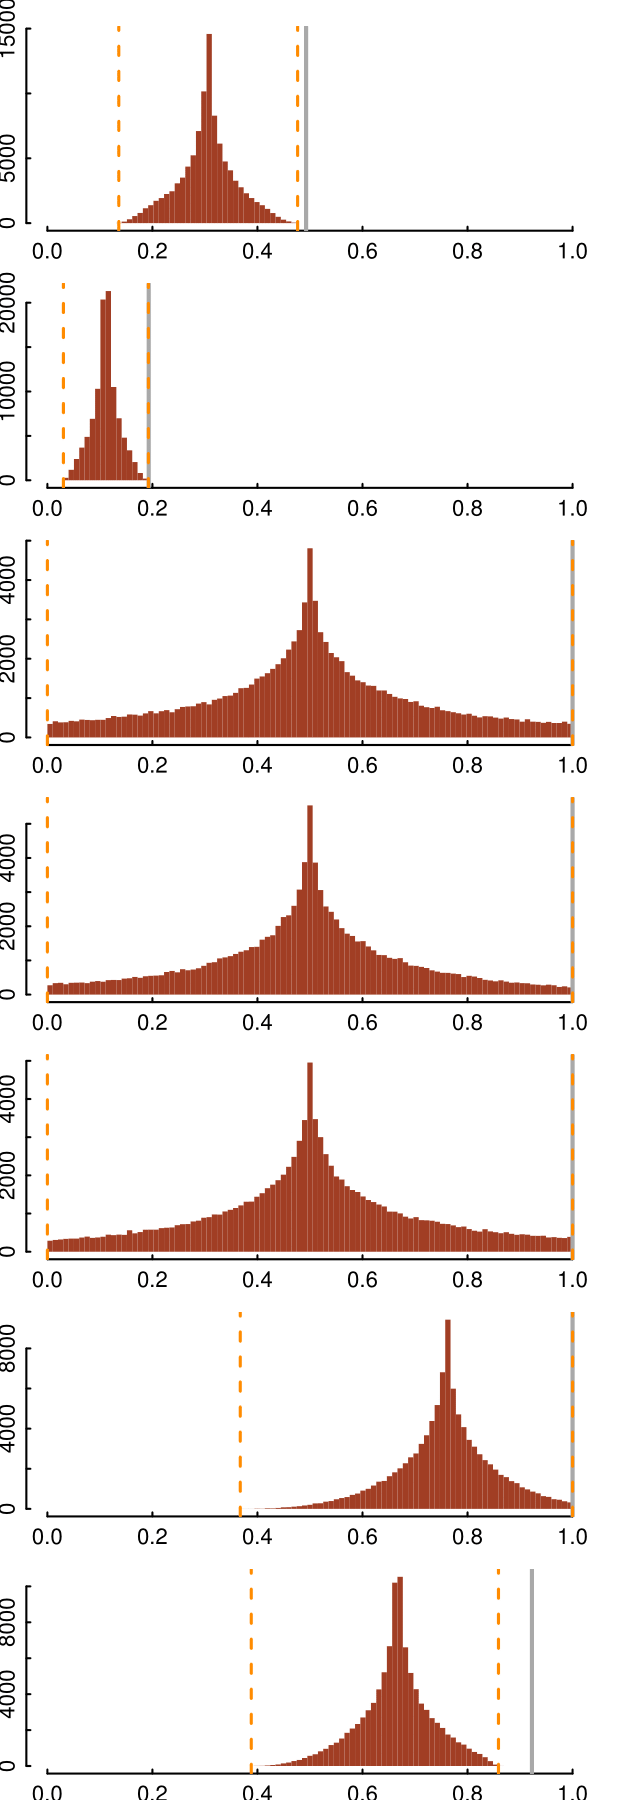
\includegraphics[width=7.5cm\textwidth]{sections/figs/raw_histograms.png}
\caption{Distribution of feasible activations for 50\% maximal force output in the palmar direction.}
\label{fig:raw_histograms}
\end{figure}


\section{RESULTS}

Figure \ref{fig:raw_histograms} shows the distributions of activations resulting from $1,000,000$ iterations of the Hit-And-Run algorithm. To our knowledge, this is the first time we can see the internal structure of the feasible activations for a sub-maximal force.

Notice also that the lower and upper bounds of the activations (i.e., the dashed lines that indicate their bounding box), are uniquely uninformative of the actual density of distribution of feasible activations. Note also that the activation needed for the maximal force output (thick gray line) is very often not the mode of the activations at 50\% of output.

